\lab{Application}{Stochastic Cake-Eating Problem}{Stochastic Cake-Eating Problem}
\newcommand\ve{\varepsilon}

\objective{In this section we study the stochastic cake-eating problem with both normal and AR(1) shocks.}

\section*{Infinite Horizon, Stochastic, i.i.d.}\label{SecRecProbInfinHorStochiid}

In practice, dynamic programming problems often involve some level of uncertainty.
For example as time progresses prices may fluctuate, resources may vary, or preferences themselves may change.
 In this lab, we reexamine the cake eating problem, this time allowing for uncertainty.

We consider again the problem of optimizing a sequence of decisions over an infinite time horizon.
We assume that the individual's preferences deviate each period according to some ``shock" $\ve$,
where $\ve$ is a random variable.  We assume that the shock terms $\ve$ for each time period are
independent and identically
distributed (i.i.d.).  In effect, this means the probabilities associated with the $\ve$ are the
same for any time $t$ and do not depend on each other.  We assume for now that the $\ve$ are
distributed normally with mean $\mu$ and variance $\sigma^2$.  The Bellman equation can be easily
rewritten in the following way to incorporate the uncertainty,
\begin{equation}\label{stoch_Bellman}
   V\left(W,\ve\right) = \max_{W'\in[0,W]}\: \{\ve u\left(W - W'\right) +
   \beta E_{\ve'}\left[V\left(W',\ve'\right)\right]\},
\end{equation}
where $\ve \sim N(\mu,\sigma^2)$ and
$E$ is the unconditional expectation operator over $\ve$.  Note that now the value function depends
on two variables.  It represents the value of entering the period with $W$, the amount of cake,
and a preference shock of $\ve$.  For example, in a period where the realization of $\ve$ is higher,
we will get more value from the cake eaten in the current period.  Because we do not know the value of
the shock in the next period $\ve'$, we consider only the expected value for future time.

It turns out, we can solve this problem in a manner similar to the infinite horizon deterministic cake-eating
problem considered in the Value Function Iteration lab.  It is worth noting that in this case,
 the value and policy functions will be two dimensional as they will depend on both $W$ and $\ve$.

In order to deal with $\ve$ computationally, we would like to represent it as a vector of possible values
it could take along with the corresponding probabilities that it takes each of those values.  However,
$N(\mu,\sigma^2)$ is a continuous distribution, so we cannot represent every value $\ve$ could take.
We need a discrete distribution that approximates $N(\mu,\sigma^2)$.

To do this, we choose $N$ equally spaced points centered about the mean, at which to approximate the
distribution. Call these values $\ve_1,\ldots,\ve_N$, and let the spacing between adjacent points be
given by $\delta$.
We can then break up the support of the distribution into $N$ bins, where adjacent bins share a common
endpoint. Call the endpoints of these bins $v_1,\ldots,v_{N+1}$. By choosing the endpoints to be
halfway between each $\ve_k$, we have the formula
\[
v_k = \ve_k - \frac{1}{2}\delta, \qquad k=1,\ldots,N
\]
and
\[
v_{N+1} = \ve_N + \frac{1}{2}\delta.
\]

\begin{figure}[h!]
\label{stoch1_fig1}
\begin{center}
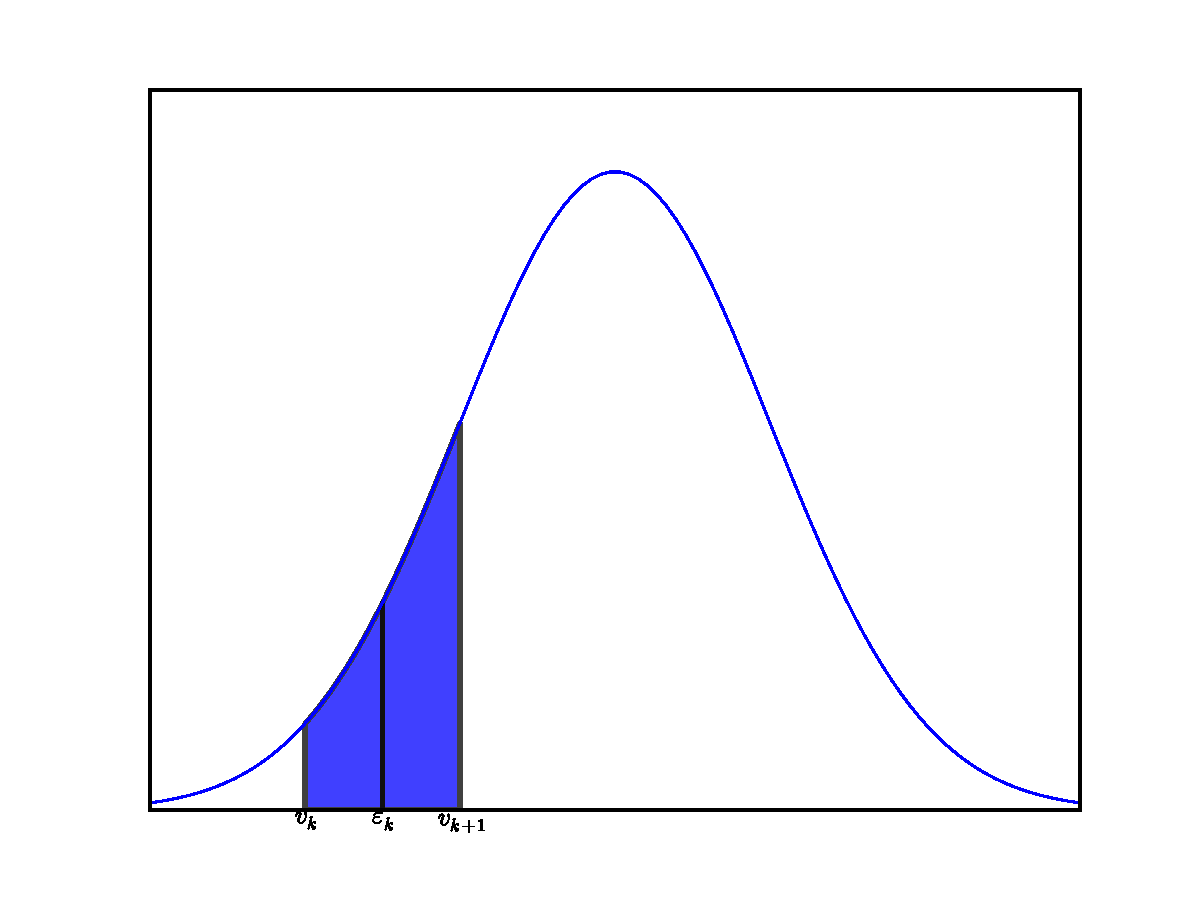
\includegraphics[width = \textwidth]{discnorm.pdf}
\end{center}
\caption{Discretization of $N(\mu,\sigma^2)$.  We approximate $P(\ve = \ve_k)$ by the area of the shaded region.}
\end{figure}

We can then associate $\ve_k$ with the area under the curve from $v_k$ to $v_{k+1}$.
In Python, we can find the area using the function \li{norm.cdf} found in the \li{stats} package.
The cdf (cumulative distribution function) gives the area under the curve from $-\infty$ to a specified value.
For example, in the following code, \li{eps} is the area under the curve from 0 to 1.

\begin{lstlisting}
>>> from scipy import stats as st
>>> mu = 0
>>> sigma = 1
>>> eps = st.norm.cdf(1,loc=mu,scale=sigma) - st.norm.cdf(0,loc=mu,scale=sigma)
\end{lstlisting}

In general, it is sufficient to take our points $\ve_k$ ranging from $\mu - 3\sigma$ to $\mu + 3\sigma$, as this
range contains about 99.7\% of the probability mass.

\begin{problem}
Write a function called \li{discretenorm} that accepts an integer $K$ representing the number of discrete points
desired, a mean $\mu$, and a standard deviation $\sigma$. It should return a length-$K$ vector of equally-spaced
values ranging from $\mu - 3\sigma$ to $\mu + 3\sigma$ inclusive,
and a length-$K$ vector containing the associated probabilities.
Plot the approximation of $N(0,1)$ using different values of $K$ to check that your results are plausible.
\end{problem}

Now that we have a discrete distribution for $\ve$, we can solve for the value and policy functions
determined by \eqref{stoch_Bellman}.

\begin{problem}
Complete the following steps to solve the problem described above.
Assume that the period utility function is $u(c)=\sqrt{c}$.
Write a function \li{stochEatCake}
that accepts parameters $\beta$ (discount factor), $N$ (number of discrete cake values),
a tuple of values \li{e_params}, $W_{max}$ (the original size of the cake, set to default value 1),
a keyword argument \li{iid} (set to default value \li{True}), and
a keyword argument \li{plot} (set to default value of \li{False}). Inside the function, carry out the steps
outlined below.

The argument \li{e_params} is a tuple consisting of the values needed to generate
the discrete approximation to $\ve$. In the present case, this tuple consists (in order) of
$K$ (the number of discrete approximations of $\ve$), $\mu$ (the
mean of the shock term $\ve$), and $\sigma$ (the standard deviation of the shock term $\ve$),
since these are the arguments we need to pass to our \li{discretenorm} function.

\begin{enumerate}
\item First, compute an approximation of $\ve$ using the \li{discretenorm} function created in Problem 1.
Use $K$ equally spaced points to approximate $N(\mu,\sigma^2)$. Denote the resulting $K$-length
vector of equally-spaced values by
\[e =(e_1,\ldots,e_K),
\]
and denote the $K$-length vector of the associated probabilities
by
\[\Gamma = (\Gamma_1,\ldots,\Gamma_K).
\]
Note that $\Gamma_k$ give the probability $P(\ve = e_k)$.

Since the values needed for the \li{discretenorm} function are contained in the \li{e_params} input,
we can feed these values directly into the function in the following way:
\begin{lstlisting}
>>> e, gamma = discretenorm(*e_params)
\end{lstlisting}
The \li{*} operator essentially unpacks the values of a tuple or list.

\item As in the Value Function Iteration lab, create a vector
\[w = (w_1,\ldots,w_N)
\]
of possible cake sizes. This should be
a length-$N$ vector of equally spaced values from 0 to $W_{max}$, inclusive.

\item Represent the value function as a $N \times K$ matrix $v$, satisfying
\[
v_{i,j} = V(w_i, e_j).
\]
(The rows correspond to different values of $W$ and the columns correspond to different values of $\ve$.)
Initialize each entry of the matrix to 0.

Likewise, represent the policy function as a $N \times K$ matrix $p$, satisfying
\[
p_{i,j} = \psi(w_i,e_j).
\]
Initialize all entries to 0.

\item In order to evaluate the value function equation, we need to pre-compute $\ve u(W-W')$ for all values of
$\ve,W,W'$.
Begin by computing all possible values of $u(W-W')$, and storing these values in a $N \times N$ array,
as in the Value Function Iteration lab. Call this array $u$. Make sure that the upper triangular
entries of this array are equal to zero, as these entries correspond to consuming more cake than is
available, which is impossible.

The values $\ve u(W-W')$ will be represented by a three-dimensional array $\hat{u}$ of size
$N\times N\times K$, satisfying
\[
\hat{u}_{i,j,k} = v_{i,j}e_k.
\]
We can compute this array easily as follows:

\begin{lstlisting}
>>> import numpy as np
>>> u_hat = np.repeat(u, K).reshape((N,N,K))*e
\end{lstlisting}


\item We also need to compute $E_{\ve'}\Bigl[V\left(W',\ve'\right)\Bigr]$ for each value of $W'$.
The expected value is simply
\begin{equation*}
E_{\ve'}\Bigl[V\left(W',\ve'\right)\Bigr] = \sum_{k=1}^K \Gamma_kV(W',e_k').
\end{equation*}
The result is length $N$ vector, call it $E$, satisfying
\[
E_i = E_{\ve'}\Bigl[V\left(w_i,\ve'\right)\Bigr] = \sum_{k=1}^K \Gamma_kv_{i,k}
\]
This calculation can be done by multiplying $\Gamma$ element-wise to each row of the
value function matrix $v$, and then summing along the rows. Something like the following
line of code should do the trick:
\begin{lstlisting}
>>> E = (v*gamma).sum(axis=1)
\end{lstlisting}

\item We can now compute the value function contraction
\begin{equation*}\label{EqContractStochiid}
C\Bigl(V\left(W,\ve\right)\Bigr) \equiv \max_{W'\in[0,W]}\:
\Bigl\{\ve u\left(W-W'\right) + \beta E_{\ve'}\Bigl[V\left(W',\ve'\right)\Bigr]\Bigr\}.
\end{equation*}
The first task is to create a $N \times N \times K$ array $c$ satisfying
\[
c_{i,j,k} = \hat{u}_{i,j,k} + \beta E_j.
\]
This can be done in any manner of ways. Below is a one-liner that does the job.
\begin{lstlisting}
>>> c = np.swapaxes(np.swapaxes(u_hat, 1, 2) + beta*E, 1, 2)
\end{lstlisting}

Now, for any $k$ and $i < j$, set $c_{i,j,k}$ to a large negative number, say $-10^{10}$,
so that when maximizing over this array, we do not choose to consume more cake than is available.
Again, this can be done in a variety of different ways, but the following does the job concisely:
\begin{lstlisting}
>>> c[np.triu_indices(N, k=1)] = -1e10
\end{lstlisting}

Finally, maximize over the second axis of $c$ (which corresponds to different values of $W'$)
to obtain the updated value function matrix:
\begin{lstlisting}
>>> v_new = np.max(c, axis=1)
\end{lstlisting}
You can likewise update your policy function matrix as follows:
\begin{lstlisting}
>>> max_indices = np.argmax(c, axis=1)
>>> p = w[max_indices]
\end{lstlisting}

\item We now have our updated value function matrix $v_{new}$ as well as the
previous $v$, which we refer to here as $v_{old}$. As we iterate on the value function equation, we need a norm
\begin{equation*}
\delta = \|v_{new} - v_{old}\|_2
\end{equation*}
that measures the distance between these two value functions to determine convergence.
You may compute the norm using the SciPy function \li{scipy.linalg.norm}, or by direct calculation.
At the end of each iteration, make sure to set $v$ to $v_{new}$, so that the updates carry through the
loop.
Iterate on the contraction until $\delta < 10^{-9}$.

\item If \li{plot = True}, make a 3-D surface plot of the policy function for the converged problem
$W' = \psi\left(W,\ve\right)$ which gives the value of the cake tomorrow as a
function of the cake today  and the taste shock today.  Do the same for the value function.
Example code to create the value function plot is provided below.
\begin{lstlisting}
>>> x = np.arange(0,N)
>>> y = np.arange(0,K)
>>> X,Y = np.meshgrid(x,y)
>>> fig1 = plt.figure()
>>> ax1 = Axes3D(fig1)
>>> ax1.plot_surface(w[X], Y, v.T, cmap=cm.coolwarm)
>>> plt.show ()
\end{lstlisting}
Creating the policy function plot is similar.

\item Return the converged value function matrix $v$ and policy function matrix $p$.


\end{enumerate}
Test your function using values $\beta = .9$, $N = 100$, $K = 7$, $\sigma = .5$, $\mu = 4\sigma$,
and \li{plot = True}.
The proper way to set this up and call the function is as follows:
\begin{lstlisting}
>>> e_params = (7, 4*.5, .5)
>>> stuff = stochEatCake(.9, 100, e_params, plot=True)
\end{lstlisting}
\end{problem}

\begin{figure}
    \centering
    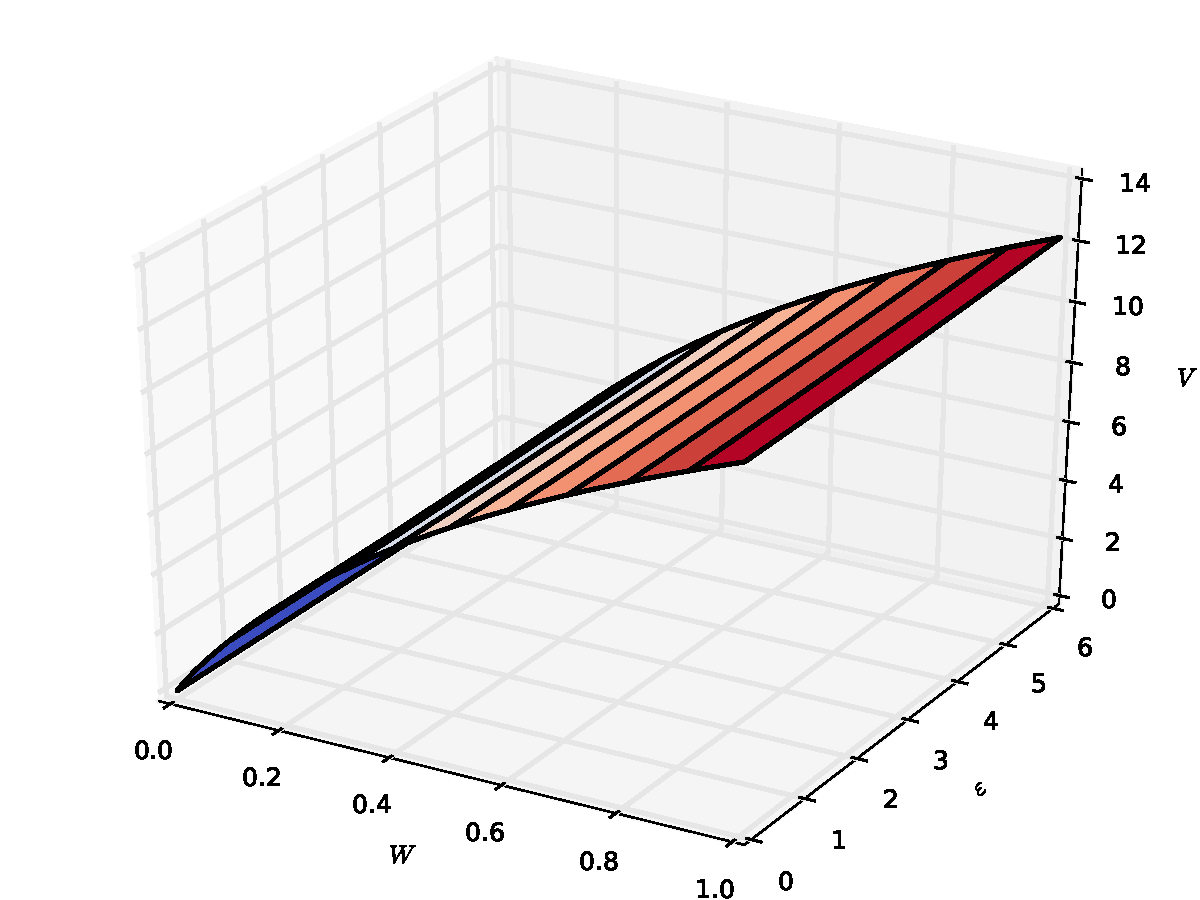
\includegraphics[width = \textwidth]{stoch_value.pdf}
    \caption{3D surface representing the value function for the Stochastic Cake-Eating problem.}
\end{figure}

\section*{Infinite Horizon, Stochastic, AR(1)}\label{SecRecProbInfinHorStochAR1}

In the previous example, we assumed that the shocks at time $t$ were independent of what happened in
previous periods.  Often a shock may depend on recent events.  We will assume now that the shocks are persistent,
meaning preferences in the current period are more likely to be close to what they were in the previous period.
We can characterize the persistence by what is called an autoregressive process of order one, denoted AR(1).
Such a process is defined as follows.
\begin{equation}\label{EqAR1shock}
\ve' = (1-\rho)\mu + \rho\ve + \nu' \quad\text{where}\quad \rho\in(0,1) \quad\text{and}\quad \nu\sim N(0,\sigma^2).
\end{equation}

Essentially, instead of allowing the shocks to have a mean which is independent of the past, the mean is now a
weighted average (weighted by $\rho$) of some $\mu$ and the previous realization of the shock, $\ve$.  As it turns
 out, we can approximate this process by thinking of it as a Markov Chain. This means we need to determine a
 discrete set of points representing possible values of $\ve$ and a Markov transition matrix that gives the
 probabilities of moving from one value of $\ve$ to another.  There are methods for determining the discrete
 approximation of $\ve$ with a Markov transition matrix.  These methods are beyond the scope of this section,
 but you can use the file \li{tauchenhussey.py} to implement them in the next problem.

The Bellman equation becomes the following, in which the only change from the i.i.d. shock case is that the
expectations operator is now conditional on the current shock $\ve$:

\begin{equation*}
   V\left(W,\ve\right) = \max_{W'\in[0,W]}\: \{\ve u\left(W - W'\right) +
   \beta E_{\ve'|\ve}\left[V\left(W',\ve'\right)\right]\},
\end{equation*}
where $\ve'$ is distributed according to \eqref{EqAR1shock}.
Let $\Gamma_{i,j}=P\left(\ve_j'|\ve_i\right)$ where $\ve_j'$ is the value of the shock in
the next period and $\ve_i$ is the value of the shock in the current period.
In other words, $\Gamma$ is the Markov transition matrix.

The solution to this problem is of the same type as that in the i.i.d. case, since the only difference is
the probability distributions of the $\ve$.

\begin{problem}
Expand your \li{stochEatCake} function to handle the case of AR(1) shock terms. The function should
handle this case for the parameter value \li{iid = False}, and should handle the previous case of
normally distributed i.i.d. shock terms for the parameter value \li{iid = True}. You will need to
add a few ``if ... else" statements, as well as implement the steps outlined below, but most of the
code will remain unchanged.

\begin{enumerate}
\item In the AR(1) case, the \li{e_params} argument should be a tuple of values needed to
generate the arrays $e$ and $\Gamma$ that approximate the values and distribution of $\ve$
as a Markov chain.
Use the file \li{tauchenhussey.py} to calculate these arrays.
The provided Python function \li{tauchenhussey} produces the vector $e$ of length $M$
and an $M\times M$ transition matrix $\Gamma$.
Thus, you simply need the following lines of code, similar to the previous case.
\begin{lstlisting}
>>> from tauchenhussey import tauchenhussey
>>> e, gamma = tauchenhussey(*e_params)
\end{lstlisting}

\item Because our values for $e$ and $\Gamma$ are different in the AR(1) case than
in the i.i.d. case, we must compute the expectation in a different manner.
In particular, we need to compute the conditional expectation
\begin{equation*}
E_{\ve'|\ve}\Bigl[V\left(W',\ve'\right)\Bigr].
\end{equation*}
We obtain a two-dimensional array, since the expectation depends on both $W'$ and on $\ve$.
The expectation can be computed by the matrix multiplication $v\Gamma^T$.
Your code should match the following.
\begin{lstlisting}
>>> E = v.dot(gamma.T)
\end{lstlisting}

\item The last difference comes in computing the array $c$. Fortunately, it is easier in this case.
Recall that $c$ gives the values for
\[
\ve u\left(W-W'\right) + \beta E_{\ve'|\ve}\Bigl[V\left(W',\ve'\right)\Bigr].
\]
The array $\hat{u}$ contains the values for the first term in the expression, and the array $E$
contains the values for the expectation term.
Hence, we obtain $c$ by simple addition. Array broadcasting makes this work without problems.
\begin{lstlisting}
>>> c = u_hat + beta*E
\end{lstlisting}
You will still need to set the upper triangular entries of $c$ to a large negative number, just as in the
previous case.
\end{enumerate}

Those are the only differences. Let the following code snippet be a guideline for how to implement
these differences.
\begin{lstlisting}
>>> if iid:
>>>     # compute E as outlined in problem 2
>>> else:
>>>     # compute E as outlined in the current problem
\end{lstlisting}

Now test your function with $\beta = .9$, $N = 100$, \li{iid = False}, and \li{plot = True}.
As inputs to \li{tauchenhussey}, let $K=7$, the mean of the process
$\mu=4\sigma$, $\rho = 1/2$, $\sigma=1/2$, and
\[baseSigma=(0.5+\frac{\rho}{4})\sigma +
(0.5 - \frac{\rho}{4})\frac{\sigma}{\sqrt{1-\rho^2}}.
\]
Your \li{e_params} parameter will therefore be a tuple of values containing (in order)
$K$, $\mu$, $\rho$, $\sigma$, and $baseSigma$.
\end{problem} 